%%%%%%%%%%%%%%%%%%%%%%%%%%%%%%%%%%%%%%%%%%%%%%%%%%%%%%%%%%%%%%%%%%%%%%
% This layout was adapted from one found at latextemplates.com which
% was adapted from another.
%
% License: CC BY-NC-SA 3.0
% (http://creativecommons.org/licenses/by-nc-sa/3.0/)
%
% Original header:
%
% This is a LaTeX version of the sample laboratory report from
% Virginia Tech's copyrighted 08-09 CHEM 1045/1046 lab manual.
% Reproduction of this one appendix section for academic purposes
% should fall under fair use.
%
%%%%%%%%%%%%%%%%%%%%%%%%%%%%%%%%%%%%%%%%%%%%%%%%%%%%%%%%%%%%%%%%%%%%%%

\documentclass{article}

\usepackage{graphicx} % Lets us use images
\usepackage[acronym]{glossaries} % Lets us use acronyms

\author{Charles Pittman}
\title{ELEC-311\\ Project 1\\ Combinational Circuit Analysis}
\date{September 17, 2013}

\loadglsentries{acronyms} % Actually loads 'acronyms.tex'
\makeglossaries

\begin{document}

\maketitle % Inserts title, author, and date from above

\pagebreak

% Removes indentation from paragraphs: \setlength\parindent{0pt}

% Number the enumerate environment (unordered lists) by letter:
\renewcommand{\labelenumi}{\alph{enumi}.}

\section{Objective}
\label{sec:objective}

% Multiple objectives:
 \begin{description}
 \item[First Objective] \hfill \\
   Analyze a combinational logic circuit and determine its behavior.
 \item[Second Objective] \hfill \\
   Use the Xilinx ISE Design Suite to simulate the logic circuit and
   program a \gls{fpga} board to verify the behavior.
 \end{description}

\section{Discussion}
\label{sec:procedure}

Lorem ipsum dolor sit amet, consectetuer adipiscing elit. Donec
hendrerit tempor tellus. Donec pretium posuere tellus. Proin quam
nisl, tincidunt et, mattis eget, convallis nec, purus. Cum sociis
natoque penatibus et magnis dis parturient montes, nascetur ridiculus
mus. Nulla posuere. Donec vitae dolor. Nullam tristique diam non
turpis. Cras placerat accumsan nulla. Nullam rutrum. Nam vestibulum
accumsan nisl.

\section{Results}

\begin{table}[h]
  \label{tab:table_01}
  \centering
  % This LaTeX table template is generated by emacs 24.3.1
  \begin{tabular}{cccc|c}
    $I_0$ & $E$ & $I_1$ & $S$ & $Z$ \\
    \hline
    0 & 0 & 0 & 0 & 0 \\
    0 & 0 & 0 & 1 & 0 \\
    0 & 0 & 1 & 0 & 0 \\
    0 & 0 & 1 & 1 & 0 \\
    0 & 1 & 0 & 0 & 0 \\
    0 & 1 & 0 & 1 & 0 \\
    0 & 1 & 1 & 0 & 0 \\
    0 & 1 & 1 & 1 & 1 \\
    1 & 0 & 0 & 0 & 0 \\
    1 & 0 & 0 & 1 & 0 \\
    1 & 0 & 1 & 0 & 0 \\
    1 & 0 & 1 & 1 & 0 \\
    1 & 1 & 0 & 0 & 1 \\
    1 & 1 & 0 & 1 & 0 \\
    1 & 1 & 1 & 0 & 1 \\
    1 & 1 & 1 & 1 & 1 \\
  \end{tabular}
  \caption{Truth table: $E \cdot (\overline{S} \cdot I_0 + I_1) \cdot (I_0 + S \cdot I_1)$}
\end{table}

% Insert a picture.  The file was "./img/plot1.png".  The LaTeX
% compiler is finicky sometimes about filenames and extensions.  I
% think it depends on what compiler is actually being used.
%\begin{figure}[h]
%  \centering
%  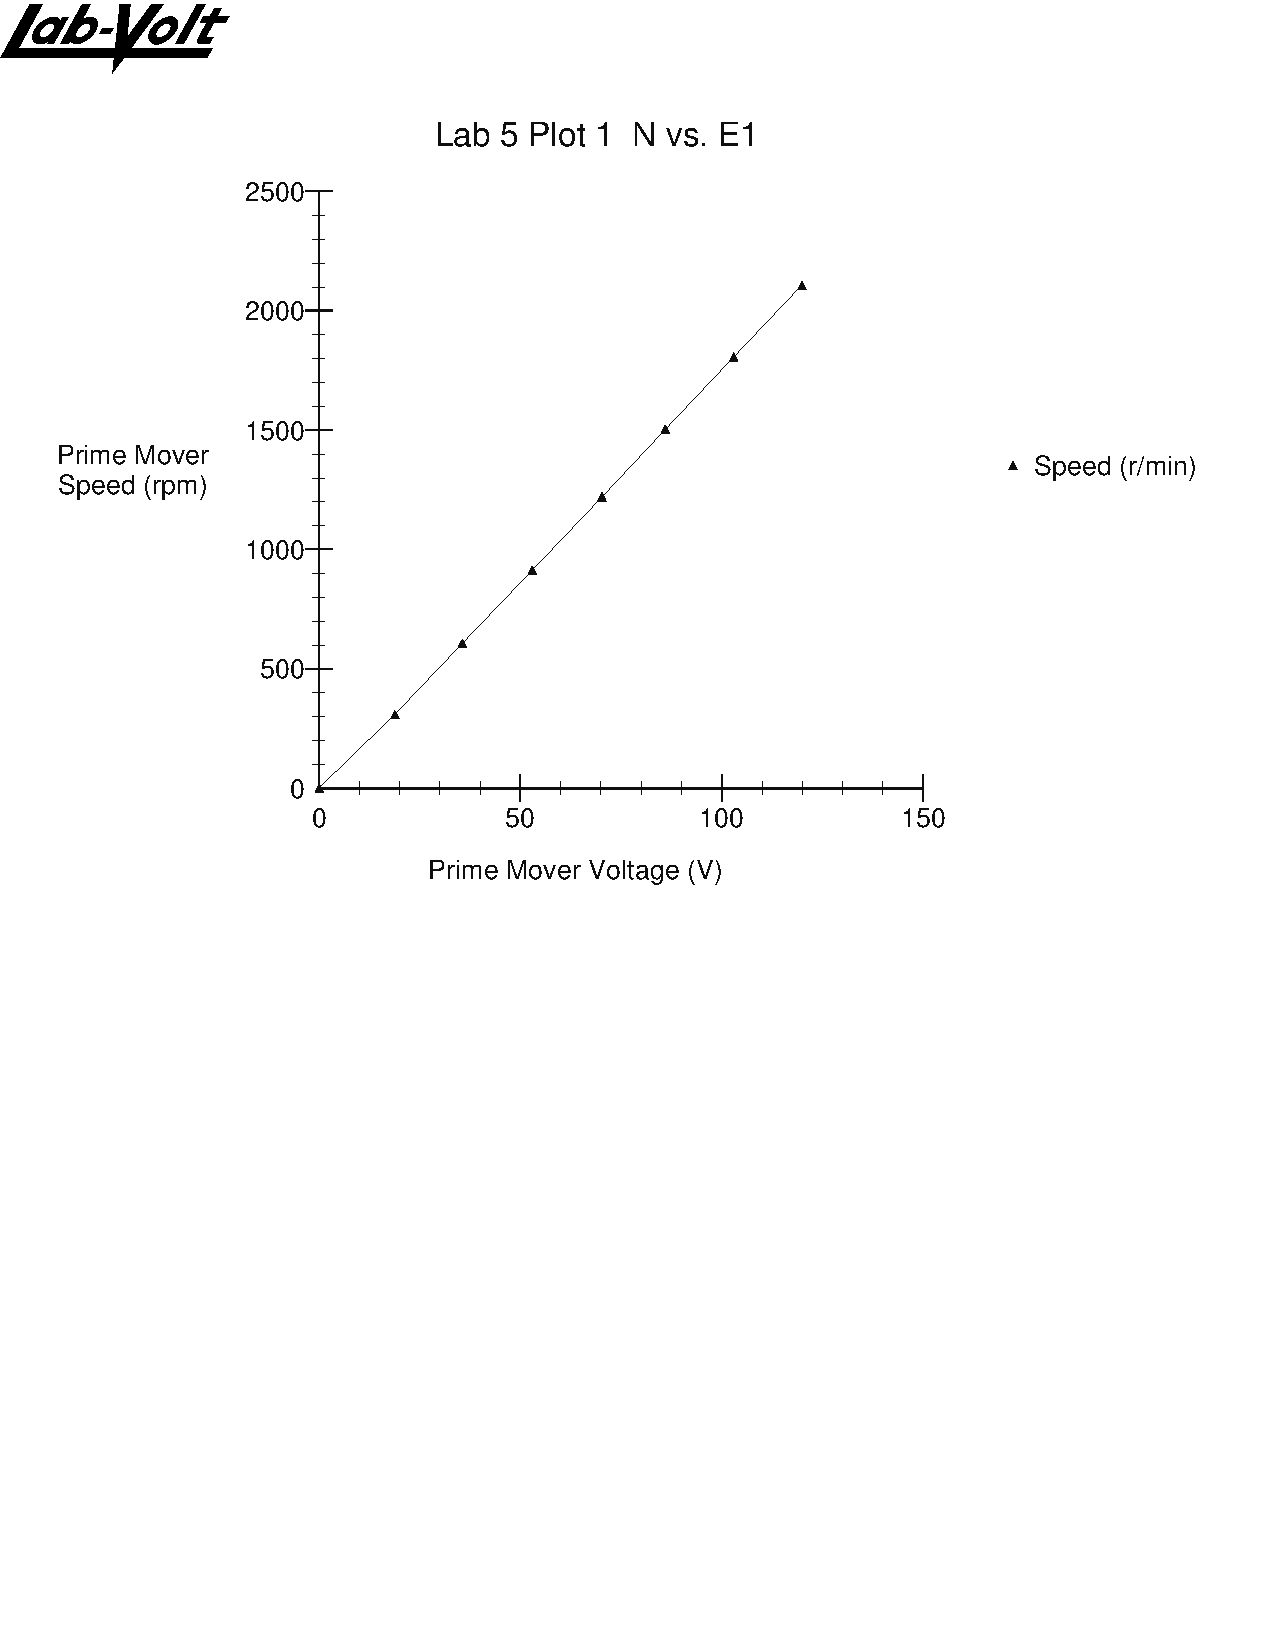
\includegraphics[width=\textwidth]{img/plot1}
%  \caption{\gls{pm} Speed vs. \gls{pm} Voltage}
%  \label{fig:plot_01}
%\end{figure}

\section{Conclusions}
\label{sec:conclusion}

Nullam eu ante vel est convallis dignissim. Fusce suscipit, wisi nec
facilisis facilisis, est dui fermentum leo, quis tempor ligula erat
quis odio. Nunc porta vulputate tellus. Nunc rutrum turpis sed
pede. Sed bibendum. Aliquam posuere. Nunc aliquet, augue nec
adipiscing interdum, lacus tellus malesuada massa, quis varius mi
purus non odio. Pellentesque condimentum, magna ut suscipit hendrerit,
ipsum augue ornare nulla, non luctus diam neque sit amet
urna. Curabitur vulputate vestibulum lorem. Fusce sagittis, libero non
molestie mollis, magna orci ultrices dolor, at vulputate neque nulla
lacinia eros. Sed id ligula quis est convallis tempor. Curabitur
lacinia pulvinar nibh. Nam a sapien.

\end{document}
